\documentclass[12pt, a4paper]{article}

\usepackage[margin=5em]{geometry}
\usepackage{graphicx}

\setlength\parskip{1em}
\setlength\parindent{0em}

\title{Assignment 3}

\author{Hendrik Werner s4549775}

\begin{document}
\maketitle

\section{Paper}
I chose the paper "Data types à la carte":

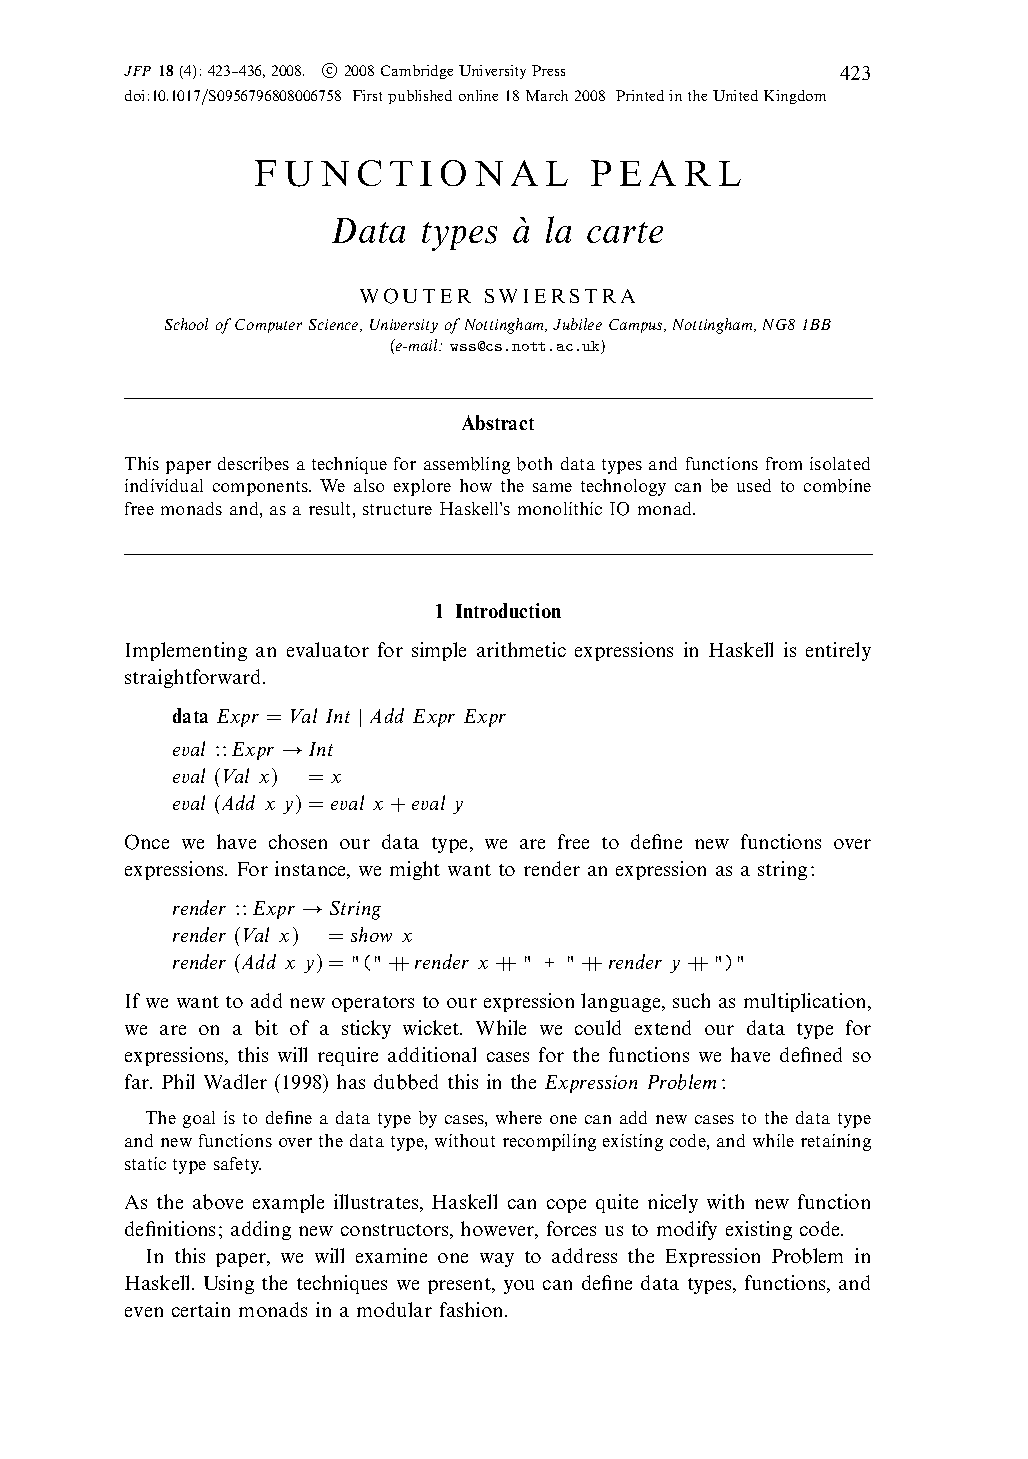
\includegraphics[page=1]{DataTypesALaCarte}

\section{Target Audience}
The article is targeted at advances functional programmers and language designers, especially those familiar with Haskell.

The author uses advanced (functional) programming terms without explanation (monolithic, monads, \dots). Also the article's topic is not generic, so that people not familiar with the matter will not be able to understand the content, nor would it be useful to them if they did.

\section{Message}
The article presents methods for solving the Expression Problem. To this end the author first introduced the Expression Problem, explains why it is indeed a problem, and then presents a solution to this problem. He then discusses the implications and importance of his approach.

\section{Effectiveness of the Introduction}
The introduction does a good job of presenting the Expression Problem and telling the reader what the rest of the paper is trying to achieve. There is even a short example program given, illustrating the problem, which I really like. This takes away much of the abstractness of the topic. The example is small, self contained, and easy to understand.

\end{document}
